

\documentclass{acm_proc_article-sp}
\usepackage{float}% If comment this, figure moves to Page 2
\usepackage{epstopdf}
\usepackage{pstricks}
\usepackage{graphicx}
\usepackage{placeins} 
\begin{document}

%\title{A Sample {\ttlit ACM} SIG Proceedings Paper in LaTeX
%Format\titlenote{(Does NOT produce the permission block, copyright information nor page numbering). For %use with ACM\_PROC\_ARTICLE-SP.CLS. Supported by ACM.}}
\title{GPSInsights: An efficient framework for storing and mining massive real-time vehicle location data}

\subtitle{[Extended Abstract]
%\titlenote{A full version of this paper is available as
%\textit{Author's Guide to Preparing ACM SIG Proceedings Using
%\LaTeX$2_\epsilon$\ and BibTeX} at
%\texttt{www.acm.org/eaddress.htm}}
}
%
% You need the command \numberofauthors to handle the 'placement
% and alignment' of the authors beneath the title.
%
% For aesthetic reasons, we recommend 'three authors at a time'
% i.e. three 'name/affiliation blocks' be placed beneath the title.
%
% NOTE: You are NOT restricted in how many 'rows' of
% "name/affiliations" may appear. We just ask that you restrict
% the number of 'columns' to three.
%
% Because of the available 'opening page real-estate'
% we ask you to refrain from putting more than six authors
% (two rows with three columns) beneath the article title.
% More than six makes the first-page appear very cluttered indeed.
%
% Use the \alignauthor commands to handle the names
% and affiliations for an 'aesthetic maximum' of six authors.
% Add names, affiliations, addresses for
% the seventh etc. author(s) as the argument for the
% \additionalauthors command.
% These 'additional authors' will be output/set for you
% without further effort on your part as the last section in
% the body of your article BEFORE References or any Appendices.

\numberofauthors{3} %  in this sample file, there are a *total*
% of EIGHT authors. SIX appear on the 'first-page' (for formatting
% reasons) and the remaining two appear in the \additionalauthors section.
%
\author{
% You can go ahead and credit any number of authors here,
% e.g. one 'row of three' or two rows (consisting of one row of three
% and a second row of one, two or three).
%
% The command \alignauthor (no curly braces needed) should
% precede each author name, affiliation/snail-mail address and
% e-mail address. Additionally, tag each line of
% affiliation/address with \affaddr, and tag the
% e-mail address with \email.
%
% 1st. author
\alignauthor
Tobin%\titlenote{Dr.~Trovato insisted his name be first.}\\
       \affaddr{Institute for Clarity in Documentation}\\
       \affaddr{1932 Wallamaloo Lane}\\
       \affaddr{Wallamaloo, New Zealand}\\
       \email{trovato@corporation.com}
% 2nd. author
\alignauthor
G.K.M. Tobin%\titlenote{The secretary disavows
%any knowledge of this author's actions.}\\
       \affaddr{Institute for Clarity in Documentation}\\
       \affaddr{P.O. Box 1212}\\
       \affaddr{Dublin, Ohio 43017-6221}\\
       \email{webmaster@marysville-ohio.com}
% 3rd. author
\alignauthor Lars Th{\o}rv{\"a}ld%\titlenote{This author is the
%one who did all the really hard work.}\\
       \affaddr{The Th{\o}rv{\"a}ld Group}\\
       \affaddr{1 Th{\o}rv{\"a}ld Circle}\\
       \affaddr{Hekla, Iceland}\\
       \email{larst@affiliation.org}
}
% There's nothing stopping you putting the seventh, eighth, etc.
% author on the opening page (as the 'third row') but we ask,
% for aesthetic reasons that you place these 'additional authors'
% in the \additional authors block, viz.
\additionalauthors{Additional authors: John Smith (The Th{\o}rv{\"a}ld Group,
email: {\texttt{jsmith@affiliation.org}}) and Julius P.~Kumquat
(The Kumquat Consortium, email: {\texttt{jpkumquat@consortium.net}}).}
\date{30 July 1999}
% Just remember to make sure that the TOTAL number of authors
% is the number that will appear on the first page PLUS the
% number that will appear in the \additionalauthors section.

\maketitle
\begin{abstract}
Intelligent Transport System (ITS) has seen growing interest in collecting various types of location-based data of transport vehicles in circulation in order to build up high quality real-time traffic monitoring system. However handling those massive and continuous data remains a challenge. In this paper, we have proposed GPSInsights, an automated system for effectively processing massive data stream produced by GPS vehicle tracking equipments. GPSInsights is built on open-source, scalable and distributed frameworks. We also have demonstrated our system with a scalable map matching implementation and perform experiments with big dataset. 

% A category with the (minimum) three required fields
\category{H.4}{Information Systems Applications}{Miscellaneous}
%A category including the fourth, optional field follows...
\category{D.2.8}{Software Engineering}{Metrics}[complexity measures, performance measures]

\terms{Bigdata}

\keywords{GPSInsights, spatio-temporal data storage, distributed data processing, map matching}
\end{abstract}

\section{Introduction}


With the widespread adoption of GPS technology, Intelligent Transport System~(ITS) has seen growing interest in collecting location-based data of transport vehicles. This data collection is done with the purpose of being able to deliver not only real-time traffic monitoring but also useful traffic statistics and predictive information. Lee et al.~\cite{Lee2011} a data mining algorithm to discover traffic bottlenecks. Demiryurek et al.~\cite{Demiryurek2010} proposed an online computation of optimal traffic route based on traffic data. None of these approaches discuss how to implement the system at large-scale.


According to Decree No. 91/2009/ND-CP of Ministry of Transport of Vietnam, all Vietnamese-licensed cars in must be equipped with a standardised global positioning system (GPS) (black-box) which reports geo-location, speed and direction every 30 seconds to a centralised data center. With nearly 200.000 cars in circulation in the near future, the data is enormous and has big data characteristics. First, data is generated continuously in big volume (e.g. petabytes (PB)) from hundred thousand of vehicles. Second, in-coming data rate is near real-time, at which the underlying system must deliver. Third, data has big value for the potential insights about the current situation of the traffic infrastructure as well as for the predictions. 


As big data create non-conventional challenges, current ITS management systems storing data in relational database systems (e.g. via PostGIS~[ref]) will not be able to adapt to the data ingestion rate, nor being able to be processed efficiently. In this work, we describe GPSInsights: a novel scalable system for storing and mining massive real-time vehicle location data. GPSInsights is able to handle increasingly huge volume of data (~PB) while supporting real-time analytics. We demonstrates GPSInsights with a scalable map matching implementation. 

This paper is organised in 7 parts. In Section~2, we discuss an overall architecture of our system framework. In Section~3, we go into the details of the technologies and components of GPSInsights. In Section~4, we establish a simple demonstration map matching algorithm. Section~5 presents experimental results for the algorithm presented in Section~4. Section~6 discusses related works on existed map matching algorithms and on storing spatio-time data. We conclude and discuss future work in Section~7.
	
\section{System design} 
	
%After being sent continuously from moving vehicles to converging data centers (note), the transportation information data will be pulled into a data mining block. The data mining block will process, analyze them and then send statistic results to a visual display system through a connect module. The general system design is illustrated as follow:

%\begin{figure}[!htb]
%\centering
%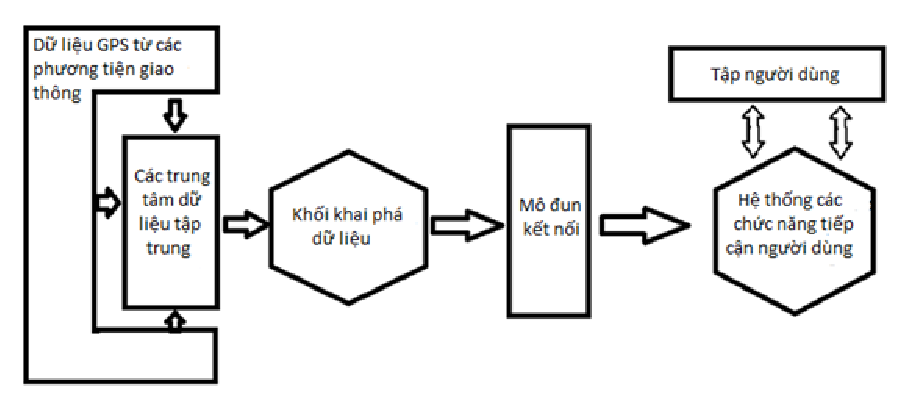
\epsfig{file=thesis-1.eps, height=140px, width=250px}
%\caption{The architecture of the system}
%\end{figure}

%As a massive amount of transportation data being directed to these centers per second, the data mining block has to have following requirements.

%We design GPSInsights with the following goals: 
%\begin{itemize}
%\item	The collected data are put in their order of arrival in time, and all of them have to be processed at least one.
%\item	The processing time is acceptable. With a quantity of data, the processing time  must not exceed than the collecting one.
%\item  Final statistic results have to be saved for using later.
%\end{itemize}

%In order to 
%meet with the above requirements and deal with the challenges of big volume, velocity, it is necessary to construct the data mining %block as a scalable system with scalable components as follows.

We design GPSInsights with the following components as depicted  in Figure~[ref]:

\begin{itemize}
\item 	Distributed message queue: As the location data come continuously from a huge number of source vehicles, this component is designed to combine the multi-source data, and put them in their chronological order. It has to store and replicate the large input data dispersedly on a large cluster for high-throughput, and fault-tolerance. The distributed message queue implements producer-consumer skeleton in which GPS devices installed on transportation vehicles are the producers and the storage engine or the processing engine of GPSInsights become the consumers.

\item  Streaming data processing engine: To allow realtime analytics, GPSInsights powers a streaming data processing engine. This component has to be able to analyse data "on the fly", which then outputs analytic reports such as average speed, number of vehicles, and traffic bottleneck prediction. It has to be scaled out on thousand of servers to adapt to the workload.

\item  Distributed result queue: Results from the data processing engine are sent to this component. This acts as the interface to continuous consumer services at application level such as web, mobile apps. 

\item  Distributed spatio-temporal database: As location data consist of geolocation information and timestamp in which the data is recorded, GPSInsights stores data in a distributed spatio-temporal database. This components aims to provide the spatial querying and data manipulation as PostGIS but at large-scale for offline phase. 

\item  Distributed analytic result database. This database is selected to store the analytic results from the data processing engine, acting as the datastore for both display services at the application level and offline processing systems. 

\end{itemize}


\section{Implementation} 

With the system architecture shown in Chapter~2, we build our GPSInsights on open-source components with custom plugins to satisfy our design goals . By leveraging existing components, we can develop GPSInsights quickly and focus on the scalable aspect of the entire system. A part of our contribution is then about designing the system overall,  carefully choosing the right components, and running the experiments with real datasets.  

\begin{figure}[!htb]
\centering
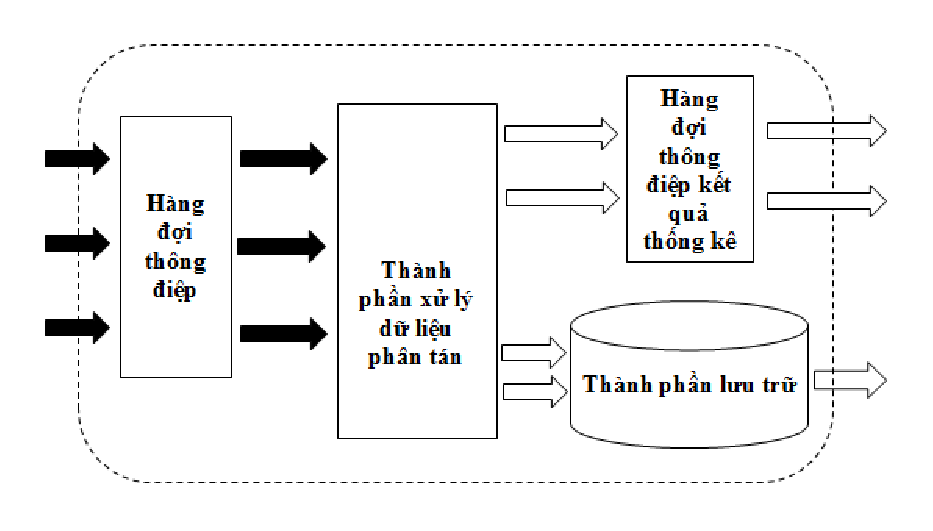
\epsfig{file=thesis-2.eps, height=125px, width=250px}
\caption{The architecture of the system}
\end{figure}

\subsubsection{Distributed message queue: Apache Kafka~[ref].} Apache Kafka is the distributed publish-subscribe messaging. Kafka stores the data in categories called topic. A topic will be divided into one or more partitions which be distributed over nodes of a cluster (each partition is an ordered, immutable sequence of messages). It allows store the amount of the data larger than the capability of any single machine. Internally, each record of the data called a "message", uniquely specified by an id number called "offset" which is its ordinal number in a partition. 
Reading to and writing data in topic are very fast, thanks to paralleling operations and several useful techniques installed to maximize the performance. According to Kafka's official website, a single Kafka broker can handle hundreds of megabytes of reads and writes per second from thousands of clients.
Kafka is designed to allow transparently and easily expanded without downtime. Kafka also can replay any message or set of messages given the necessary selection  criteria. In addition, partitions are persisted on disk and replicated within the cluster to prevent data loss. So Kafka offers strong scalable, durability and  fault-tolerance.

\subsubsection{Streaming data processing engine: Spark Streaming~[ref] and Storm~[ref].}
Spark Streaming and Apache Storm now are the most popular open-source frameworks for distributed stream processing. However, there are important differences in their architectures as following.

Spark Streaming is a module of Apache Spark for acting on data stream as soon as it arrives. It provides an abstraction called Dstreams (discretized streams). A Dstream is represented as a continuous sequence of data arriving over time. More detail, a set of data arriving at each time step, received by a component called "receiver", will be packed in a batch called an RDD, so each Dstream is a continuous sequence of RDDs. An RDD is simply an immutable distributed collection of objects. We cannot change any property of an object in RDD. Using Map-Reduce model, Each RDD is split into multiple partitions, which may be processed by "executors" on different nodes of a Spark Streaming cluster. Each operation on partition of RDD is also executed in memory, so running programs on Spark Streaming is very fast. According to Spark's official website, by comparison with the time of executing a logistic regression in Hadoop, running time in Spark is 100 times faster.
Spark's RDDs also offer a strong fault-tolerance , because the input data are replicated to other nodes of the cluster (In Spark 1.1 and earlier, received data was replicated in-memory only, so it could also be lost if Spark Streaming crashed. Since Spark 1.2, received data are also persisted to a reliable file system like HDFS so that they are not lost anymore), and an RDD remembers the lineage of deterministic operations that were used on that data to create it. If any partition of an RDD is lost due to a node failure, as long as a copy of the input data is still available, then that partition can be re-computed from it using the lineage of operations. So that Spark Streaming provides better support for processing each batch exactly once.

Instead of batching up events that arrive within a short time and then processing them like Spark Streaming, Storm processes incoming events one at a time (so storm’s processing latency could be sub-second, while Spark Streaming reaches a latency of several seconds). The work in Storm is delegated to different types of components that are responsible for a specific processing task. The input data stream are received by a specialized component called a "spout". Then the spout immediately passes the data to another component called a "bolt". In a bolt, the data will be transformed in some way, and the bolt either sends it to some sort of storage or passes it to some other bolt. In short, a Storm cluster can be considered as a network of bolt components in which each one applies some kind of transformation on the data receiving from the spout, the arrangement of spouts and bolts and their connections in the cluster is called a topology. In storm, each individual record has to be tracked when moving through the system. However, Storm only guarantees that each record will be processed at least once.

In GPSInsights, we mainly focus on Spark Streaming. The purpose of installing Storm as the streaming data processing engine is to compare the performance of the system when using the two frameworks to solve the same problem. The results of the comparison are expressed in the Experimental Evaluation section.


\subsubsection{Distributed result queue: Apache Kafka.} Providing a very high-throughput, Apache Kafka is relatively suitable for this position. The data processing engine will use Kafka's producer to push the statistic result data to a Kafka's topic in parallel. According to the benchmark experiments of the Kafka's developing team,  Kafka managed to write more 2 million records (approximately 193.0 MB)  per second on three cheap machines (https://engineering.linkedin.com/kafka/benchmarking-apache-kafka-2-million-writes-second-three-cheap-machines). Hence, with a suitable hardware configuration, the data processing engine can just spend a negligible time for writing the result data to the Kafka's topic. The data processing engine then continues the next input data, while the connect module uses Kafka's consumer to pull that data and send to every visual display systems of clients. This helps the data processing engine minimize the waiting time of sending the result data to external component.



\subsubsection{Distributed analytic result database: MongoDb~[ref].}
Because of the rapid increase in velocity and volume of the result data, traditional relational databases are no longer adequately suitable for such type of data. Especially as they do not scale well to very large sizes (their scaling is vertical; more data means a bigger server) and large data solutions become very expensive using relational databases. NoSQL (not only SQL) databases like mongoDB become an outstanding candidate for big data storing. Firstly, NoSQL databases have been designed to provide good horizontal scalability for read/write database operations distributed, as well as  have the ability to replicate and to distribute data, over many servers. These multiple servers can be cheap commodity hardware or could instances, it is a lot more cost effective than vertical scaling of relational databases. Secondly, being divorced from normal table relationships and constraints, as well as ACID (atomicity, consistency, isolation, and durability) of data for increasing the performance, their read/write operations are very faster than the traditional databases. 
The result storage is used to store the big-volume and high-velocity statistic results from the data processing engine. Hence, we need a distributed data storage. It also has the ability to write data fast in order to avoid increasing the processing time of the data processing engine. So that mongoDb – the most popular NoSQL database is selected for this position.

\subsubsection{Distributed spatio-temporal database: Geomesa~[ref].}
 GeoMesa~\cite{fox2013spatio} is an open-source, distributed, spatio-temporal database  built on top of a column-family oriented distributed database called Accumulo~\cite{accumuloonline}. GeoMesa uses a very flexible strategy to linearize geo-time data and distribute the data across the nodes in a cluster to leverage parallelism in computationally intensive queries. It enables efficient storing, querying, and transforming capabilities for large spatio-temporal data. Furthermore, GeoMesa supports open OGC APIs, which facilitates transition from other databases to this database. This database provides specialized functions for manipulating the spatial-temporal data like which is similar to PostGIS's functions, adding advantages of NoSQL database. It is very suitable for storing and querying the raw input data for offline phase in the future. So why not use Geomesa as the distributed analytic result database? There are several reasons for this. Firstly, the output data from the streaming data processing engine do not include the spatial field like latitude and longitude, so that we cannot take advantage of the spatio-temporal database. Secondly, Geomesa does not support update operation which we will need for improving the system in later.  Finally, Geomesa has not supported for receiving the data from Apache Spark yet. Hence, we have to use a Geomesa basic function to d
o this, it is enormously slow.


One other reason of choosing the distributed message queue as a component of GPSInsights is to minimize the number of data which loss while recovering from failures. In the case without the message queue component, the transportation data are sent directly to the data processing engine. If a master node of a Spark Streaming cluster dies or "Spout" component of a Storm cluster crashes, they cannot receive any data which arrive during this time. By contrast, if the number of failure node is smaller than the number of nodes keeping the input data (for example, if received data are replicated across two nodes, the queue can tolerate single node failures), the queue always receive the arrival data in spite of the failures of the data processing engine. When recovering, the data processing engine continues pulling the unprocessed data from the queue and then handling them.

However, after successful connecting between different components of GPSInsights, we realized that there were some inherent problems in the system. Firstly, the system could not guarantee that the output data from Spark Streaming were completely sent to MongoDb. This happened when Spark Streaming went wrong, while pushing the result data to the result database. MongoDb in this case just received the incomplete set of the data, but Spark Streaming supposed it completed the task with the current batch and then continued handling the following batch. Hence, that there would be some records which will be lost in the failure case.

\begin{figure}[!htb]
\centering
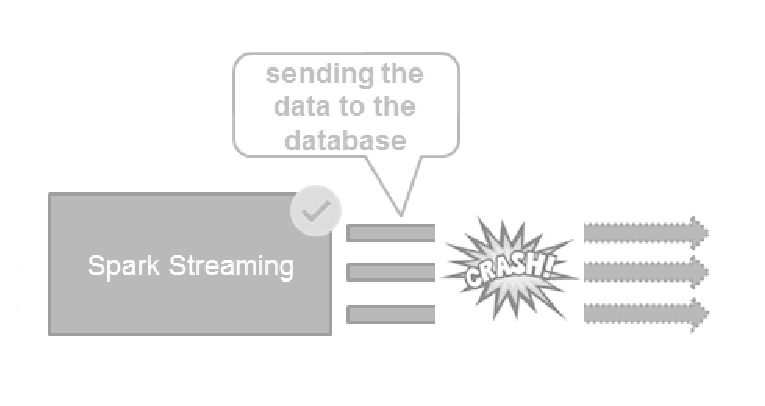
\epsfig{file=thesis-3.eps, height=100px, width=220px}
\caption{The first problem}
\end{figure} 

Secondly, some records might appear repetitively in a batch due to failures. Because after the received data are replicated persistently on HDFS, the Spark Streaming Receiver informed Kafka about this, so the problem can occur when a part of received data are saved on the reliable filesystem, but Spark Streaming failed before updating for Kafka. Therefore, Spark Streaming supposed it received the data, but Kafka supposed that the data was not sent successfully. So Kafka would resend the data after the streaming data processing engine recovered from the failure.

 
\begin{figure}[!htb]
\centering
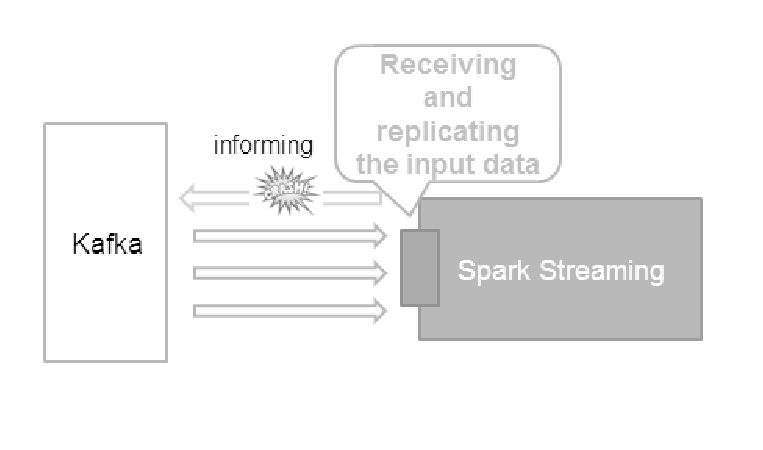
\epsfig{file=thesis-4.eps, height=100px, width=220px}
\caption{The second problem}
\end{figure} 

The cause of the above problems is that each component of GPSInsights cannot know exactly whether the data are handled fully by the other component or not. To overcome these, only one component needs to maintain a consistent view of what has been processed successful by the system. Therefore, we decided to build a transaction of writing the result data to MongoDB. It means that either all output data from Spark Streaming are logged to MongoDB or the arriving data are reprocessed by the system. 

To build this, firstly, we rewrote Spark Streaming's Receiver by using Spark Streaming's "receiverStream" API and Kafka's Simple Consumer API [* ref link] to take advantage of the Kafka's ability of replaying the data from arbitrary offsets.  Instead of only handling the latest data when using the old Receiver, with the new one, we can arbitrarily specify any start position of the offset for each partition at the beginning of every batch interval. Besides, we can get the extra information of each record including its offset, id of the partition which it belongs to.  Secondly, we created a MongoDb database with three different collections namely "Transactions", "Records", "OffsetRanges". "Transaction" includes documents have three fields: id, timestamp and status. There are two value of status field, "BEGIN" means the beginning of a transaction and "FINISH" expresses the end of the transaction. "Records" contains documents which are the information of the analytic results from Spark Streaming and an id of the transaction. "OffsetRanges" includes documents which hold the information of an offset range of the records packaged into the current batch, and the id of the transaction.

The detail implementation will be described as follows. Before sending to Spark Streaming's Receiver, each record in Kafka will be attached with its offset and partition's id which it belongs to. Using Accumulator API [* ref link], we can find the offset range of each Kafka's partition in the current batch. When finishing handling this batch, before logging the result data to MongoDb, we create a new document with "Begin" status in "Transactions" collection and get its id. We then create a new document in "OffsetRanges" collection with the offset range and the id. Next, we send the result data to "Records" collection, attaching the id. Finally, after the last record is written successful in MongoDb, we change the status field of the transaction to "Finish", and the current batch is handled successful. During running, if the system fails and then recovers, it will query MongoDb for the last document in "Transactions" collection.  If the value of the status field is "Finish", it means the process of handling the last batch was succeeded. By contrast, we will use the transaction id to get the relevant document in "OffsetRanges" collection, and use the first offset in each ranges (the number of range is equal to the number of partition of the Kafka' topic that we are consuming) to recomputed the data. 

\section{Demonstration: Scalable map matching}
\subsection{Dataset}
Our data include about 12,565,521 GPS records collected by vehicles equipped with a GPS receiver from 22/03/2014 to 22/04/2014 in Ho Chi Minh city. Every record consists of speed, GPS coordinate and state of the vehicle and the period of time between two records is 15 minutes. The following table shows the format of the data.

\begin{table}[h]
\centering
\begin{tabular}{|c|c|c|c|c|}
\hline
\textbf{time\_stamp} & \textbf{car\_id} & \textbf{lon}   & \textbf{lat} & \textbf{speed} \\ \hline
\end{tabular}
\end{table}

\subsection{Algorithm: Road Reverse Geocode Algorithm Using K-D Tree.}	
	
\subsubsection{Process OSM raw data.}
	The Open Street Map's raw data consist of a mass of tag almost covering the whole world. Every node tag has some tags inside to determine its attributes (e.g. type, way's name, coordinate, ..). Way tag contains one or more node tags that used to define the shape of it.
	
		\setlength{\parindent}{0.7cm} Before going to the details, vertices, links and segments should be defined clearly. Link is a section of road between intersections. In most digital maps, a real road is digitized and is described with a set of many straight lines. Vertices are points which separate these straight lines, and each straight line is a segment. The road AD in Fig.~\ref{fig:composition} is formed by 3 intersections (black points), 2 vertices (white points), 2 links (AD, DE) and 3 segments(AB, BC, CD).
		
\begin{figure}[h]
\centering
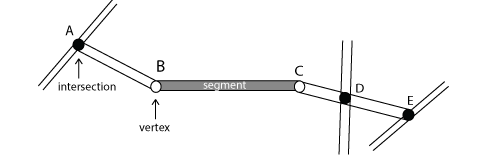
\includegraphics[height=100px,width=210px]{figure1}
\caption{The composition of the road network}
\label{fig:composition}
\end{figure}
	
		\setlength{\parindent}{0.7cm} Our purpose is to determine all links and their information (name of roads which contain these links). Firstly, we traverse the tag list of OSM, read all Way tags, ignore irrelevant ways (roads that are unfit for transports such as cars, taxis and buses) and then store all associated node ids (we use BTree for this task). If a node occurs once, it is a vertex. Otherwise, it is an intersection. Secondly, we store all Node tags for later uses.
	
\subsubsection{Link matching.}
	
	Because the transport data are collected from GPS tracking device, the input consists of a sequence which contains a time stamp and a geographic coordinate. Our task is to assign a GPS point to a relevant link. Kd-tree is chosen to tackle this problem~\cite{moh2013approximate}. It is an efficient searching method to quickly find nearest points and this algorithm only takes O(log n) average time per search in a reasonable model.
	
	\setlength{\parindent}{0.7cm} Despite the fact that the standard deviation of GPS data could be quite low in the best case, around 3 meters, it can increase several fold due to tree cover, tunnel and other problems. The limited sampling polling time intervals is the second source affecting the accuracy. There are many methods to solve quite effectively this, including vertex-based and segment-based map matching, map matching using the geometric relationship, map matching using the network topology, the data history and so forth. This paper does not focus on this problem, we only use the vertex-based map matching for the simplicity of the process.  
	
%	\begin{figure}
%		\subfloat[vertex-based map matching]{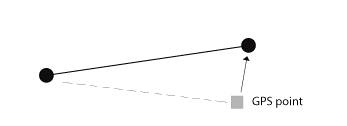
\includegraphics[width = 0.5\linewidth]{figure3}} 
%		\subfloat[Add some equidistant vertices in segments]{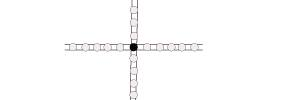
\includegraphics[width = 0.5\linewidth]{figure2}\label{fig:sfig2}}
%	\caption{Link matching}
%	\end{figure}
	
	\setlength{\parindent}{0.7cm} We go through the list of ways in OSM and add some equidistant vertices in segments ( illustrated in Fig.~\ref{fig:sfig2}) and build a KD-Tree based on those vertices. Note that a node in the Kd-Tree consists of a coordinate and information of a link which associates it. Therefore, by taking a GPS point into the Kd-Tree and using the vertex-based map matching, we can determine its nearest vertex as well as a link it is matched to.
	
	\subsubsection{Describe our algorithm.}
		
	\setlength{\parindent}{0.7cm} In this section, we focus on explaining our proposed algorithm in traffic volume statistic. With this algorithm, we query vehicle object q in a specific time period and a GPS bound from Geomesa aimed at achieving following attributes of q: q's latitude, q's longitude and q's speed. All the information we will store in a data structure list – input. After getting input data from Geomesa, now, we review how Spark is used in our algorithm. Firstly, we build up a kdTree with OSM data preprocessed and then broadcast it to the nodes in our system (Line 14). By doing this, we can keep a read-only variable cached on each machine instead of shipping a copy of it with tasks, thereby, providing every node a copy of the kdTree which make up a lot of memory and construction time. Secondly, it is necessary for our algorithm to utilize a collection in-parallel in order to construct a distributed dataset from input data list which can be operated on in paralle. Because the parallel collection can be used many times, we will cache it on memory accelerating our program (Line 15).
	
\setlength{\parindent}{0.7cm} As we have a parallelized collection formed, our algorithm will be divided into two phase: a data mapping phase and a data collecting phase. 

\subsubsection{Data Mapping Phase:} All the elements of the parallelized collection (object q) will be passed on the maptopair method of spark which can operate on in-parallel. As every object q go into the method, the nearestPoint method of copies of kdTree cached on each machine can be utilized aimed at finding what point of a road segment (p) is nearest point of object q and how long distance between q and p (Line 19). Because of the fact that coordination GPS sent from satellites will have some deviations in comparison with the real coordinate, so that we have to choose a threshold distance in order to determine whether object q belong to the road segment including p or not (Line 20 - 27). If the distance is smaller than the threshold distance, it will be much easier for us to conclude that the object q belongs to the road segment and vice versa. As a result, our algorithm can remove the object q that its distance with the road segment is too far from, therefore, we can enhance the accuracy of our algorithm to some extent. Finally, in the Line 29, after every object q is matched to a road segment by road segment's ID, we will group the matched pairs by road segment's ID, hence, we can obtain $<$key, value$>$ pairs with key being a roadID and value being a iterable of vehicleID and speed.

\setlength{\parindent}{0.7cm} In the next step in the phase, we will continue to process the $<$key, value$>$ pairs in-parallel by using the maptopair method of spark. The number of vehicle moving on a road segment also the average speed of the road segment will be calculated in the step (Line 33 - 34).

\subsubsection{Data Collecting Phase:} In data mapping phase, statistic numbers of the road segments will be processed in-parallel on the nodes of our system, so that collecting the data perform a decisive role in our algorithm. After the figures are processed, we will use the collect method of spark to convert the parallel collection into a simple list in order to summarize the information and, therefore, we will achieve statistic numbers of traffic volume and average speed on each road segments (Line 38 - 40).


{\it The Pseudocode of Algorithm}	
\begin{verbatim}

\end{verbatim}
%
\noindent

\section{Experiments}
	GPSInsights system is set up on a cluster of HPCC super computer, consisting of 4 nodes, one master node and three slave nodes. Each cluster node is equipped with a  8-cores Intel Xeon 2.6GHz CPU, 32GB memory 
	With this configuration, we have evaluated the performance of GPSInsights, using the dataset shown in section 4.1 to simulate the stream data. Firstly, We compared the running time of the system on the different number of records with various numbers of slave nodes. Secondly, we benchmark the system using Spark Streaming against the system using Apache Storm. For all experiments, the results are reported by averaging three runs. 
	
	% 	 Suppermicro SC815TQ-600WB\\ Intel Xeon E5-2670 Processor (20M Cache, 2.6 GHz, 8 Core)\\	 32 GB DDR3 RAM\\	 2*250 GB HDD\\	 FDR 56Gbps Infiniband\\
	
	\begin{figure}
		\centering
		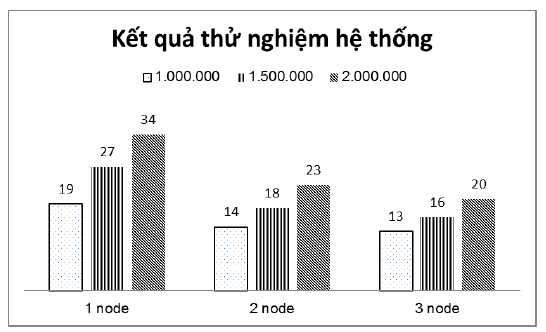
\includegraphics[height=100pt,width=150pt]{thesis-5}
		\caption{figure 5}
	\end{figure}

Figure 15 present the performance of employing GPSInsights for handling three different quantities of input records with the number of slave nodes from 1 to 3. In this experiment, the processing time of the system is measured from the time Spark Streaming pull the data from Kafka into a batch, until the analytic data of the batch are sent successful to the storage components. It is clear that the number of slave nodes was increased, the execution time of the system reduced steadily, this is thanks to the parallel procedure of Spark. Besides, we also installed a common system with Geomesa for map-matching, based on the ability of querying K-nearest neighbor search of this database, in order to have a comparison with our system. With 1.200.000 records, after 10.000 seconds running, there was no signs of stopping of the system. The performance gap between two system is mainly due to taking the advantage of Spark Streaming in our system,  we can execute the nearest neighbor search directly in memory by using the map-matching algorithm shown in section 4.2.

	\begin{figure}
		\centering
		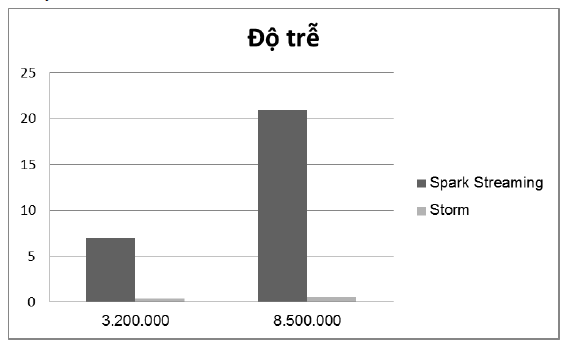
\includegraphics[height=100pt,width=150pt]{thesis-6}
		\caption{figure 6}
	\end{figure}
	
		\begin{figure}
		\centering
		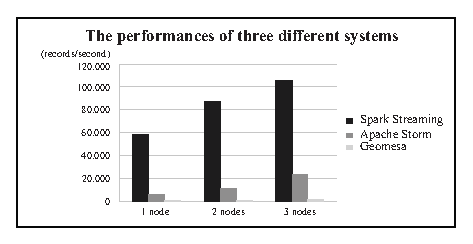
\includegraphics[height=100pt,width=150pt]{thesis-7}
		\caption{figure 5}7
	\end{figure}
	
Figure 6 and Figure 7 show the lag and the performance of two systems using two different frameworks as the streaming data processing engine for performing the map-matching algorithm in 3.200.000 and 8.500.000 records of the input data. The system using Storm beats one using Spark Streaming in term of the lag. Because Storm processes incoming events one at a time , so that its processing latency could be sub-second. Otherwise, after collecting the input data into a batch, Spark Streaming then divide it up into partitions and sent them to slave nodes. So the processing latency of Spark Streaming depends on the batch interval (if the batch interval is 5 seconds, it means that Spark has to wait 5 seconds before starting processing the first batch)  and the number of records packed in the batch (the time for sending partitions to slave nodes is directly proportional to the quantity of records). However, with the in-memory batch handling strategy, the time for processing the data of Spark Streaming is so much faster.	
	
%\section{Related work}

			
\section{Conclusion and Future Work}
This paper presents GPSInsights, a scalable, extensible and reliable system for continuously processing the massive amounts of vehicle data. We described the main components of the system, explain why to choose them, and the map-matching algorithm being inside of. We also described the method to improve the system, insuring the vehicle data which are handled exactly one, by rewriting the Spark Streaming's receiver and building the simple NoSQL transaction for MongoDb. In addition, through conducting the vehicle data statistic, we proved the GPSInsights' potential to address an increasing number of the problem classes relating massive GPS vehicle data.

In the future work, we intent to pursue the system in three directions. Firstly, We will use the advance map-matching algorithm with higher accurate on low-sampling-rate vehicle data, about 15 seconds or less. Secondly, GPSInsights will be installed new algorithm for predicting future traffic conditions based on real-time data.Finally, the system will be improved to find the fastest path depending on the travel times of each road segment.
%
% The following two commands are all you need in the
% initial runs of your .tex file to
% produce the bibliography for the citations in your paper.
\bibliographystyle{abbrv}
\bibliography{dasfaa2015}  % sigproc.bib is the name of the Bibliography in this case
% You must have a proper ".bib" file
%  and remember to run:
% latex bibtex latex latex
% to resolve all references
%
% ACM needs 'a single self-contained file'!
%
%APPENDICES are optional
%\balancecolumns
\appendix
%Appendix A
\section{Headings in Appendices}
The rules about hierarchical headings discussed above for
the body of the article are different in the appendices.
In the \textbf{appendix} environment, the command
\textbf{section} is used to
indicate the start of each Appendix, with alphabetic order
designation (i.e. the first is A, the second B, etc.) and
a title (if you include one).  So, if you need
hierarchical structure
\textit{within} an Appendix, start with \textbf{subsection} as the
highest level. Here is an outline of the body of this
document in Appendix-appropriate form:
\subsection{Introduction}
\subsection{The Body of the Paper}
\subsubsection{Type Changes and  Special Characters}
\subsubsection{Math Equations}
\paragraph{Inline (In-text) Equations}
\paragraph{Display Equations}
\subsubsection{Citations}
\subsubsection{Tables}
\subsubsection{Figures}
\subsubsection{Theorem-like Constructs}
\subsubsection*{A Caveat for the \TeX\ Expert}
\subsection{Conclusions}
\subsection{Acknowledgments}
\subsection{Additional Authors}
This section is inserted by \LaTeX; you do not insert it.
You just add the names and information in the
\texttt{{\char'134}additionalauthors} command at the start
of the document.
\subsection{References}
Generated by bibtex from your ~.bib file.  Run latex,
then bibtex, then latex twice (to resolve references)
to create the ~.bbl file.  Insert that ~.bbl file into
the .tex source file and comment out
the command \texttt{{\char'134}thebibliography}.
% This next section command marks the start of
% Appendix B, and does not continue the present hierarchy
\section{More Help for the Hardy}
The acm\_proc\_article-sp document class file itself is chock-full of succinct
and helpful comments.  If you consider yourself a moderately
experienced to expert user of \LaTeX, you may find reading
it useful but please remember not to change it.
\balancecolumns
% That's all folks!
\end{document}
